\documentclass[a4paper,ngerman,oneside,titlepage,bibliography=totoc,11pt]{scrreprt}


\pagestyle{headings}

\usepackage{geometry}
\geometry{left=31mm, top=34mm, right=31mm, bottom=34mm}

\renewcommand{\ttdefault}{lmtt}
\linespread{1.06} %font

\usepackage[font=small,labelfont=bf]{caption} %caption, caption-font
\usepackage{subcaption}

\usepackage{amsmath, amsthm, amssymb, amsbsy}
\usepackage{mathtools}
\usepackage{color}
\usepackage{booktabs}
\usepackage{svg}

\usepackage[ngerman]{babel}
\usepackage[utf8]{inputenc} % für Umlaute (ansinew Editor, utf8 bei Texniccenter/Texmaker)
\usepackage[T1]{fontenc} % korrekte Trennung von Umlauten

\usepackage[hyphens]{url}
\usepackage{hyperref}






\begin{document}


\begin{titlepage}

\newcommand{\HRule}{\rule{\linewidth}{0.5mm}} % Defines a new command for the horizontal lines, change thickness here

\center % Center everything on the page
 
%----------------------------------------------------------------------------------------
%	HEADING SECTIONS
%----------------------------------------------------------------------------------------

\LARGE Ludwig-Maximilians-Universität München\\[0.2cm] % Name of your university/college
\LARGE Institut für Statistik\\[5mm]% Major heading such as course name
\large Projekt im Rahmen des statistischen Consultings\\[6mm]
% Minor heading such as course title

%----------------------------------------------------------------------------------------
%	TITLE SECTION
%----------------------------------------------------------------------------------------

\HRule \\[0.4cm]
{ \huge \bfseries Internationaler Waffenhandel:\vspace{-1.5mm} Die Anwendung neuer Verfahren der\\[1mm] statistischen Netzwerkanalyse}\\[5mm]
{ Eine Netzwerkanalyse des internationalen Kleinwaffenhandels 1992 - 2011}\\
{ Kooperation mit dem Lehrstuhl für empirische Politikforschung}\\[0.4cm] % Title of your document
\HRule \\[1.5cm]
 
%----------------------------------------------------------------------------------------
%	AUTHOR SECTION
%----------------------------------------------------------------------------------------

\begin{minipage}[t]{0.4\textwidth}
\begin{flushleft} \large
\emph{Autoren:}\\[2mm]
Roman Dieterle\\
roman.dieterle@hotmail.de\\[5mm]

Felix Loewe\\
felixloewe@gmail.com\\% Your name
\end{flushleft}
\end{minipage}
~
\begin{minipage}[t]{0.4\textwidth}
\begin{flushright} \large
\emph{Projektpartner:}\\[2mm]
Prof. Dr. Paul W. Thurner\\[6mm]

\emph{Betreuer:}\\[2mm]
Prof. Dr. Göran Kauermann\\[6mm]
\end{flushright}
\end{minipage}\\[4.5cm]

\end{titlepage}




\begin{abstract}


\begin{center}
{\it \bf Abstract} 
\end{center}
Dieser Bericht behandelt die Analyse der \emph{NISAT database of transfers of small arms, light weapons, and their ammunition, parts and accessories}. Die Netzwerkdaten stellen das internationale Kleinwaffenhandelsnetzwerk im Zeitraum 1992 bis 2011 dar.

Nachdem die Datengrundlage besprochen wird, erfolgt eine deskriptive Analyse des Handelsnetzwerkes anhand Zeitreihen von Netzwerkstatistiken. Im zweiten Teil wird der Querschnitt des Netzwerkes Jahr für Jahr anhand von ERGMs modelliert, um charakteristische Strukturen des Netzwerkes aufzudecken. Der Fokus liegt hierbei auf der Selektion interner Netzwerkstatistiken sowie externer Kovariablen.
 \\
 
 {\bf Schlagwörter}\quad {\it Netzwerkanalyse -- Waffenhandel -- Kleinwaffen -- ERGMs}

\end{abstract}




\tableofcontents




\chapter{Einführung}

Was ist das Besondere an der statistischen Analyse von Netzwerken? Erstens stellen sie durch ihre Abhängigkeitsstruktur relationale Daten dar. Gewöhnliche Datensätze mit $i = 1, ..., N$ Beobachtungen werden zumeist mit der Annahme analysiert, dass die $n$ Beobachtungen unabhängig voneinander beobachtet werden. Bei Netzwerkdaten ist das nicht der Fall. Hier stehen die Beobachtungen, oft genannt \emph{Akteure} des Netzwerkes, in Beziehung zu einander. Besteht eine Beziehung zwischen den Beobachtungen, können diese nicht mehr als unabhängig angesehen werden. In ähnlicher Sichtweise wird auch eine nicht-bestehende Beziehungen nicht ignoriert, sondern so angesehen, dass individuenspezifische oder netzwerkspezifische Effekte diese verursacht haben können.

Das Bestehen- oder Nicht-Bestehen einer Beziehung ist die Netzwerkstruktur (\emph{Abhähngigkeitsstruktur}), die zusätzlich zu den Daten eines gewöhnlichen Datensatzes besteht. Die Abhängigkeitsstruktur wird durch die Adjazenzmatrix $Y_{ij} \in N \times N$ ausgedrückt.

Zweitens stellen Netzwerkdaten eine Verallgemeinerung von räumlichen Daten dar. Bei räumlichen Daten wird von der Nachbarschaftsstruktur gesprochen. Markov-Zufallsfelder können als Graph visualisiert werden, dessen Akteure räumliche Punkte oder zum Beispiel Länder sind.
Sind diese benachbart, besteht eine Kante. Zwei Punkte $i, j$ sind benachbart ($i \sim j$), falls der entsprechende Eintrag in der Adjazenzmatrix eine Eins aufweist. Netzwerke verallgemeinern das Konzept des räumlichen Nachbarns auf beliebige Beziehungen. Bei der Analyse des Waffenhandels wird aus der Beziehung ein Handel und aus den Akteuren die liefernden und belieferten Länder.

Die Arbeit ist wie folgt aufgebaut. Im ersten Kapitel erfolgt eine kurze Wiederholung der Begriffe aus der Graphentheorie. Diese Begriffe werden in den darauffolgenden Kapiteln verwendet, um weitere netzwerkstatistische Begriffe einführen zu können. Im zweiten Kapitel erfolgt eine Erläuterung der Datengrundlage der NISAT Datenbank. Im dritten Abschnitt wird der Datensatz deskriptiv analysiert. Im vierten Abschnitt erfolg die Modellierung per ERGMs.





\section{Wiederholung der Graphentheorie}

Um Netzwerkdaten statistisch analysieren zu können, muss die Abhängigkeitsstruktur der Daten adäquat modelliert werden. Eine grundlegende mathematische Theorie, die verwendet wird, um \emph{relationale Daten} zu beschreiben, ist die Graphentheorie. Die Notation der graphentheoretischen Begriffe orientiert sich an \cite{kc14}.

\subsection{Graph}

Ein Graph $G = (V,E)$ ist die mathematische Beschreibung eines Netzwerkes. 

Er besteht aus einer Knotenmenge $V$ und einer Kantenmenge $E$. Ein Knoten $v$ ist ein Punkt eines Graphen. Eine Kante $e$ verbindet zwei Punkte. Mit diesen zwei Begriffen kann ein Graph graphisch dargestellt werden.

Es wird eine Konvention getroffen, dass es nur eine endliche Zahl an Knoten in einem Graph gibt. Die Anzahl der Knoten wird mit $N_V = |V|$ bezeichnet. Üblicherweise sind die Knoten $v_i$ durchnummeriert mit dem Index $i = 1, ..., N_V$. 

Eine Kante $e$ ist ein Element der Menge $E$. Eine Kante $e = \{i,j\}$ beschreibt die Verbindung zwischen Knoten $v_i$ und $v_j$. 

Es gibt ungerichtete und ungerichtete Graphen. Sie unterscheiden sich darin, ob eine Kante, also die Beziehung zwischen den Akteuren, gerichtet oder ungerichtet ist. Ein Beispiel für ungerichtete Beziehungen ist eine Freundschaftsbeziehung. Ein Beispiel für eine gerichtete Beziehung ist der Kleinwaffenhandel: es gibt ein Export- und ein Importland. Das Kleinwaffenhandelsnetzwerk kann also durch einen gerichteten Graphen beschrieben werden.

Mathematisch unterscheiden sich gerichtete und ungerichtete Graphen darin, ob eine Kante $e$ ein geordnetes Paar $(i,j)$ oder ein ungeordnetes Paar $\{i,j\}$ ist. Die Kantenmenge $E$ eines gerichteten Graphs kann als Teilmenge des kartesischen Produkts $V \times V$ dargestellt werden.

Erweiterungen von Graphen stellen Graphen mit Schleifen und Multigraphen dar. Eine Schleife ist eine Kante der Form $(i,i)$. Multigraphen sind Graphen, die mehrere Kanten von einem Knoten zu einem anderen Knoten erlauben. Eine Multikante kann als Tupel $(e, r)$ definiert werden, wobei $e$ die gerichtete oder ungerichtete Kante bezeichnet, und $r$ die Anzahl der Multikanten. Um Graphen von Multigraphen zu unterscheiden, spricht man bei einem Graph ohne Multikanten von einem einfachen Graphen.

Betrachtet man die Anzahl der möglichen Kanten eines Graphen, die später als Benchmark dafür auftaucht, wie dicht ein Graph sein kann, so wird ersichtlich, dass diese Anzahl für einen einfachen ungerichteten Graphen kleiner ist als die Anzahl der möglichen Kanten einer komplizierteren Graphenart. Für einen einfachen ungerichteten Graphen ist sie gegeben durch:

$$V_H(V_H-1)/2$$

Werden Schleifen $\{i,i\}$ erlaubt, sind mehr Kanten möglich. Dann wird der Zähler durch $V_H^2$ ersetzt. Werden gerichtete Kanten $(i,j)$ erlaubt, kommen erneut mehr mögliche Kanten hinzu. Der Zähler wird dann nicht mehr durch Zwei geteilt.


\subsection{Adjazenzmatrix}

+Ein Graph ist vollständig bestimmt durch seine Adjazenzmatrix $A_{ij} \in |V| \times |V|$, wobei $a_{ij} = 1$ bedeutet, dass zwischen Knoten $i$ und Knoten $j$ eine Kante besteht.

+Bei gerichteten Graphen besteht ein Unterschied zwischen der Kante $(i,j)$ und der Kante $(j,i)$. Die Adjazenzmatrix ist dann nicht symmetrisch.


\section{Datengrundlage}

Die Datengrundlage für das Kleinwaffenhandelsnetzwerk ist die \emph{NISAT} (Norwegian Initiative on Small Arms Transfers) Datenbank. Das Peace Research Institute Oslo (PRIO) ist der Auftraggeber dieser Datenbank. Die Datenbank enthält Daten über den legalen und illegalen Handel von Kleinwaffen. Der abgedeckte Zeitraum beträgt die Jahre 1992 bis 2011.

Es folgt eine genauere Beschreibung der Datenbank. Die Daten liegen in Form von einer Edge-List vor, das bedeutet, eine Zeile steht für die gerichtete Beziehung zwischen einem Exportland und einem Importland. Diese Exportliste hat eine Reihe weiterer Kovariablen. Somit steht zur Verfügung, in welchem Jahr der Handel stattfand, welcher Waffentypus gehandelt wurde, der Waffenwert in US-Dollar und die berichtende Quelle, von dem der Eintrag stammt.

\chapter{Deskriptive Analyse}

\section{Top-Akteure}

Als erstes wird darauf eingegangen, welches die zentralen Akteure des Handelsnetzwerkes sind. Das bedeutet, es werden die Nationen aufgelistet, die über den Zeitraum von 20 Jahren das größte Import- und Exportvolumen, gemessen am Geldwert der gehandelten Waffen, aufweisen. Die Top-Exporteure sind in Tabelle \ref{top_exp} zu sehen.

\begin{table}[h]
\centering
\footnotesize
\begin{tabular}{rlr}
  \hline
 Platz & Land & Exportvolumen [Mrd.]\\ 
  \hline
1 & United States of America & 9.2\\ 
  2 & Italy & 7.9 \\ 
  3 & Germany (Federal Republic) & 4.6 \\ 
  4 & Brazil & 3.7 \\ 
  5 & Austria & 2.7 \\ 
  6 & United Kingdom & 2 \\ 
  7 & Belgium & 1.8 \\ 
  8 & Switzerland & 1.5 \\ 
  9 & Russia / USSR (Former) & 1.4 \\ 
  10 & Czech Republic & 1.4 \\ 
   \hline
\end{tabular}
\caption{Top-Exporteure des Netzwerks} 
\label{top_exp}
	\end{table}
	
Es ist ersichtlich, dass die Vereinigten Staaten von Amerika mit 10 Milliarden Dollar am meisten Waffen exportiert. Italien steht mit circa 8 Milliarden Dollar Exportvolumen an zweiter Stelle. Dies erscheint ungewöhnlich über den Zeitraum von 1992 -- 2011. Deutschland exportiert mit circa 5 Milliarden Dollar gehandelten Waffen am drittmeisten. Auf dem vierten und fünften Platz folgen die Länder Brasilien und Österreich mit exportierten Waffen, die circa 4 und 3 Milliarden Dollar wert sind. Ab dem sechsten Platz erfolgen nur noch unwesentliche Verringerungen des Exportvolumens im Bereich von 2 bis 1 Milliarde Dollar. Hierin befinden sich Nationen wie Großbritannien, Belgien, die Schweiz, Russland und die tschechische Republik. 

Nun folgt eine Auflistung der Top-Importeure des Kleinwaffenhandelsnetzwerkes (siehe Tabelle \ref{top_imp}).

\begin{table}[h]
\centering
\footnotesize
\begin{tabular}{rlr}
  \hline
 Platz & Land & Importvolumen [Mrd.]\\ 
  \hline
1 & United States of America & 16\\ 
  2 & Germany (Federal Republic) & 2.3\\ 
  2 & France & 2.3\\ 
  4 & Canada & 1.9 \\ 
  5 & United Kingdom & 1.8\\ 
  6 & Saudi Arabia & 1.7\\ 
  7 & Belgium & 1.2\\ 
  8 & Spain & 1.2\\ 
  9 & Australia & 1.2\\ 
  10 & Turkey & 1\\ 
   \hline
\end{tabular}
\caption{Top-Importeure des Netzwerks} 
\label{top_imp}
	\end{table}
		
Erneut steht Nord-Amerika an erster Stelle. Die Nation gibt circa 16 Milliarden Dolar für den Import von Kleinwaffen aus. Deutschland und Frankreich teilen sich mit 2.3 Milliarden Dollar Importvolumen den zweiten Platz am Kleinwaffenimport. Auf der vierten Stelle befindet sich Kanda mit einem Importvolumen von circa 2 Milliarden Dollar. Großbritannien verwendet 1.8 Milliarden Dollar, um Waffen zu exportieren, und Saudi Arabien 1.7 Milliarden Dollar. Auf dem siebten, achten, neunten und zehnten Platz sehen wir ähnliche Exportausgaben von circa 1.2 bis 1 Milliarde Dollar. Dies sind die Länder Belgien, Spanien, Australien und Türkei.

\section{Netzwerkmaßzahlen}

Als zweites erfolgt eine Darstellung grundlegender deskriptiver Netzwerkmaßzahlen, um das Kleinwaffenhandelsnetzwerk zu beschreiben. Die Maßzahlen werden für jedes Jahr berechnet und als Zeitreihe dargestellt, um die zeitliche Entwicklung des Netzwerkes zu visualisieren. 

\subsection{Anzahl der Knoten und Dichte}
Die ersten beiden Maßzahlen, die betrachtet werden, sind die Anzahl der Knoten und die Dichte des Netzwerkes. Je höher die Anzahl der Knoten $N_V$ im Netzwerk, desto mehr Länder sind am Waffenhandel beteiligt. Die Entwicklung der Knotenanzahl (\ref{vert_ts}) zeigt,

\begin{figure}[ht]
	\centering
  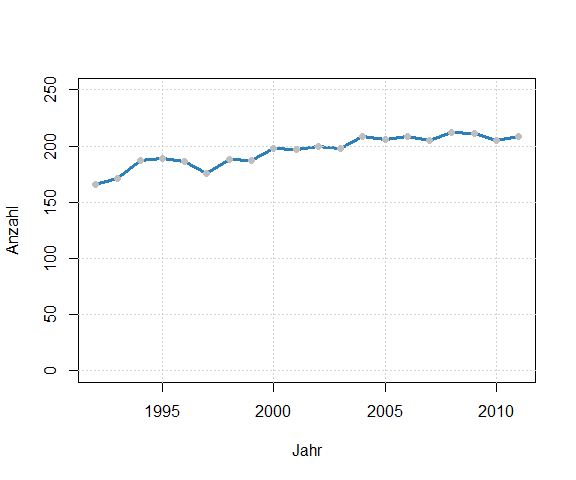
\includegraphics[scale = 1]{Grafiken/vert_ts.png}
	\caption{Knoten-Entwicklung}
	\label{vert_ts}
\end{figure}



%Die Dichte eines Netzwerkes ist die Anzahl der Kanten des Netzwerkes, geteilt durch die mögliche Anzahl an Kanten des Netzwerkes. Das Kleinwaffenhandelsnetzwerk $G_{NISAT}$ ist ein gerichteter Multigraph mit Schleifen. Da für Multigraphen keine Dichte definiert ist, wird der Graph mit dem Befehl \ttt{simplify(G_Nisat)} auf einen einfachen Graphen reduziert. Die Schleifen im Datensatz werden in der Berechnung der Dichte entfernt. Es ergibt sich der Term $den(G_{NISAT}) = \frac{E_V}{N_H(N_H-1)/2}$ für die Dichte.







 

\bibliographystyle{plain}
\bibliography{literatur}


\chapter*{Eidesstattliche Erklärung}

Wir erklären hiermit, dass wir diese Arbeit ohne fremde Hilfe angefertigt und nur die im Literaturverzeichnis aufgeführten Quellen und Hilfsmittel benutzt haben. Diese Arbeit wurde noch nicht zu anderen prüfungsrelevanten Zwecken vorgelegt.\\[1.5cm]

\noindent ................................................
\qquad\qquad\qquad\qquad\qquad
......................................................\\[0.5mm]
\textit{Ort, Datum}
\qquad\qquad\qquad\qquad\qquad\qquad\qquad\qquad\qquad
\textit{Roman Dieterle, Felix Loewe}














\end{document}


